\documentclass[a4paper]{article}

\usepackage[margin=1in]{geometry}
\usepackage{indentfirst}
\usepackage{CJKutf8}

\setlength{\parindent}{2em}
\linespread{1.5}

\title{基于深度神经网络的垃圾图像分类方法}
\author{杜楚恒}
\date{2020年8月}

\usepackage{natbib}
\usepackage{graphicx}

\begin{document}

\begin{CJK*}{UTF8}{gbsn}

\maketitle

\renewcommand{\abstractname}{摘要}
\begin{abstract}
    随着社会经济的发展,人们产生的垃圾数量飞速上涨。而垃圾分类是处理垃圾、回收资源的重要环节,可以减轻垃圾对环境的危害。传统图像分类算法已经很难满足垃圾分类的需求,而各种深度神经网络的技术,提高了垃圾分类的准确率与效率。本文基于华为垃圾分类公开数据集,以ResNet作为检测的主干网络,研究了网络深度、数据增强、注意力机制等参数和技术应用于模型的效果,提升了网络的性能。
\end{abstract}

\section{概述}

近年来,随着我国经济水平的高速发展,人们的物质消费水平不断提升,相对应的垃圾产生量也在迅速增长,由垃圾产生的问题日益突出。大量的垃圾危害着环境,但事实上,垃圾也是一种资源,绝大部分都可再回收利用,所以实行垃圾分类意义重大。
垃圾分类,是指将垃圾按照某种规则类别分别投放、保存和运输,实现资源重新利用的过程。
目前,北京、上海、广州等地纷纷推出各地的垃圾分类管理条例,将垃圾分类从居民投放到转运处理规则化,使垃圾先分入可回收、不可回收、湿垃圾、干垃圾四大类,各自转运到相关处理站点后再进行进一步的分类处理。


目前的垃圾分类,在经过大类的筛选过后,还需依靠人工分拣垃圾,生产线工作环境差、人工分拣的垃圾种类极为有限、生产效率低,导致最终能够重新利用的垃圾少之又少,不能满足日益增长的垃圾处理需求。随着深度学习技术的发展,卷积神经网络等技术使图像分类算法在精度和速度上得到了巨大的提升,让我们看到了借助视觉技术自动分拣垃圾的可能性。分拣厂可以通过拍摄垃圾图片,实时利用神经网络检测出垃圾类别,之后借助机械手或推板自动完成分拣任务,可以降低人工成本,提高分拣效率。因此,开展垃圾图像分类算法的研究,具有重要的应用价值。

% \begin{figure}[h!]
% \centering
% 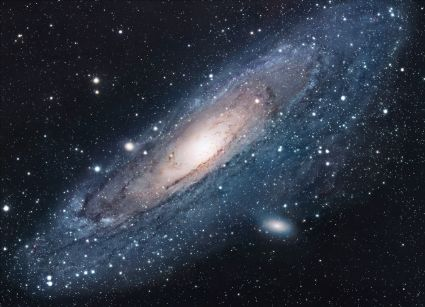
\includegraphics[scale=1.7]{universe}
% \caption{The Universe}
% \label{fig:universe}
% \end{figure}

\section{相关工作}

计算机视觉起源于上个世纪50年代,Hubel与Wiesel\cite{hubel1962receptive}发现视觉处理的前端部分不是处理图像整体,而是边缘结构,基于他们的发现,人们研究了如何从图像提取边缘结构。David Marr\cite{marr1980theory}发现视觉处理是分成不同阶段和层次的,
所以特征提取和结构划分处理成为计算机图像处理非常重要的两个课题。

人们在此基础上发明了很多常用算法: David Lowe发表在计算机视觉领域顶级会刊上的SIFT尺度不变特征算法\cite{790410},Navneet Dalal提出的HOG方向梯度直方图算法\cite{dalal2005histograms}等,但它们都或多或少依赖于模型设计者从数据中找出数据的特有结构特征,模型无法没有先验知识而直接依靠图像调整,这造成了机器学习效率与准确率一定程度上由特征选择决定,若特征选择不当,分类效果则不佳。


在早期,受到数据集规模和硬件性能的限制,深度网络参数相较于数据过于庞大,而无法有效地训练和优化。随着互联网技术与计算机硬件的发展,数据集规模有效扩大,GPU与相应加速算法的出现都使热门看到深度神经网络的未来。ImageNet(2009)是一个有1400多万张图片、涵盖2万多个类别的数据集,每年举办视觉识别挑战赛(ILSVRC)。

AlexNet(2012)是第一个崭露头角的深度神经网络: 它的深度更深; 使用Relu激活函数,缓解了梯度消失的问题; 加入了Dropout层,防止过拟合; 使用数据增强,大大增加数据集大小,增强模型对图像处理能力。之后的Clarifai(2013),GoogLeNet(2014),VGGNet(2014)都通过不同卷积层与池化层的组合实现了更好的效果。ResNet(2015)中提出了跨层链接的方法,使模型可以拥有更多卷积层。


斯坦福大学的Mindy Yang等人(2016)构建了垃圾分类数据集TrashNet Dataset,包含了6个类别: 硬纸板、玻璃、金属、纸张、塑料,总计2527张,并在其上进行初步实验,使用SVM方法\cite{yang2016classification}取得了63\%的准确率。Victoria Ruiz等人(2019)使用ResNet网络,在此数据集达到87\%的准确率; Rahmi Arda Aral等人(2018)使用DenseNet将平均准确率提升至95\%。

国内垃圾分类研究方面,向伟等(2019)使用改进的CaffeNet在识别水面垃圾上取得95.75\%的准确率。郑海龙(2019)用SVM进行建筑垃圾分类方面的研究。

\begin{figure}[h!]
\centering
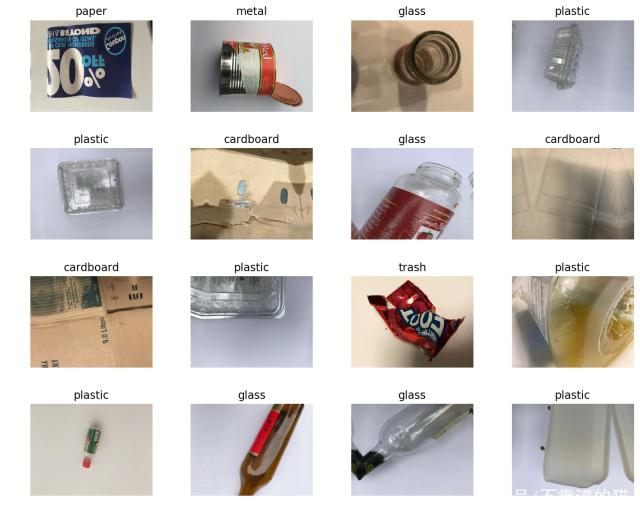
\includegraphics[scale=0.3]{trashnet_example.jpeg}
\caption{Trashnet数据示例}
\label{fig:trashnet_example}
\end{figure}

\section{垃圾分类模型}
\subsection{ResNet模型}

VGG中的卷积网络有19层,GogleNet中则达到了22层。但是,在深度学习中,网络层数增多并不一定意味着模型表现更好,过深的网络,会产生如下几个问题:

\begin{enumerate}
    \item 参数多,消耗计算资源大; 容易过拟合。可以靠增加资源和数据集大小改善。
    \item 反向传播时,回传到浅层的梯度会非常接近0,造成梯度消失,更新网络权重慢。这个问题虽然可以靠Batch Normalization得到缓解,但在实际应用中效果并不明显。
    \item 正向传播时由浅到深逐步提取图像特征,过深层网络提取的特征存在丢失信息现象。
\end{enumerate}

另一方面,虽然层数更深,但是如果浅层直接将特征复制一份传递到下一层,则层数深的网络性能不可能低于层数浅的网络。于是,残差网络的想法应运而生。何凯明等人提出的ResNet(残差网络)\cite{he2016deep}创造性地引入了跳过卷积层的连接结构Shortcut Connection,可以将输入直接越过一层或多层传递映射传递到深层,如图\ref{fig:resident_block}。在每一层中,传统深度学习得到的是输入$x$和输出$y$之间的函数 $y=\mathrm{H}(x)$,ResNet改为拟合残差函数$\mathrm{F}(x)=\mathrm{H}(x)-x$,此时的输出$\mathrm{H}(x)=\mathrm{F}(x)+x$即表示复制一份原始输入。

\begin{figure}[h!]
\centering
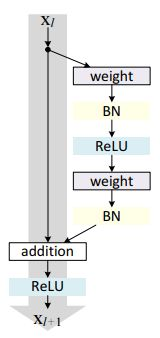
\includegraphics[scale=0.5]{resident-block.jpg}
\caption{ResNet Shortcut Connection 示例}
\label{fig:resident_block}
\end{figure}

通过复制一份输入,信息在正向传播时会一直保留原图像的特征; 在反向传播时,由于复制项的存在,计算得出的梯度不可能一直为0,梯度消失的问题也得到了很好的解决。残差网络在正向和反向的过程中,信息都可以畅通地在深层和浅层之间传递。

\subsection{注意力机制}

在人类视觉机制中,注意力机制非常关键,由于大脑处理能力有限,便将注意力集中在重点处理的区域,深度学习中的注意力机制也是如此,他使模型更加关注待识别的物体而忽略背景。在垃圾分类的数据集中,拍摄的垃圾背景十分复杂,若将背景与物体前景混为一体,将干扰模型对于垃圾的检测,故可以在模型中添加注意力机制,使网络关注于待检测垃圾。

在本次实验中采用了CBAM(Convolutional Block Attention Module)实现注意力机制,CBAM是由Sanghyun Wee等人\cite{woo2018cbam}提出的一种轻量、通用的注意力模块。该模块分为两个部分,分别为通道注意力模块和空间注意力模块,如图\ref{fig:cbam}所示。

\begin{figure}[h!]
\centering
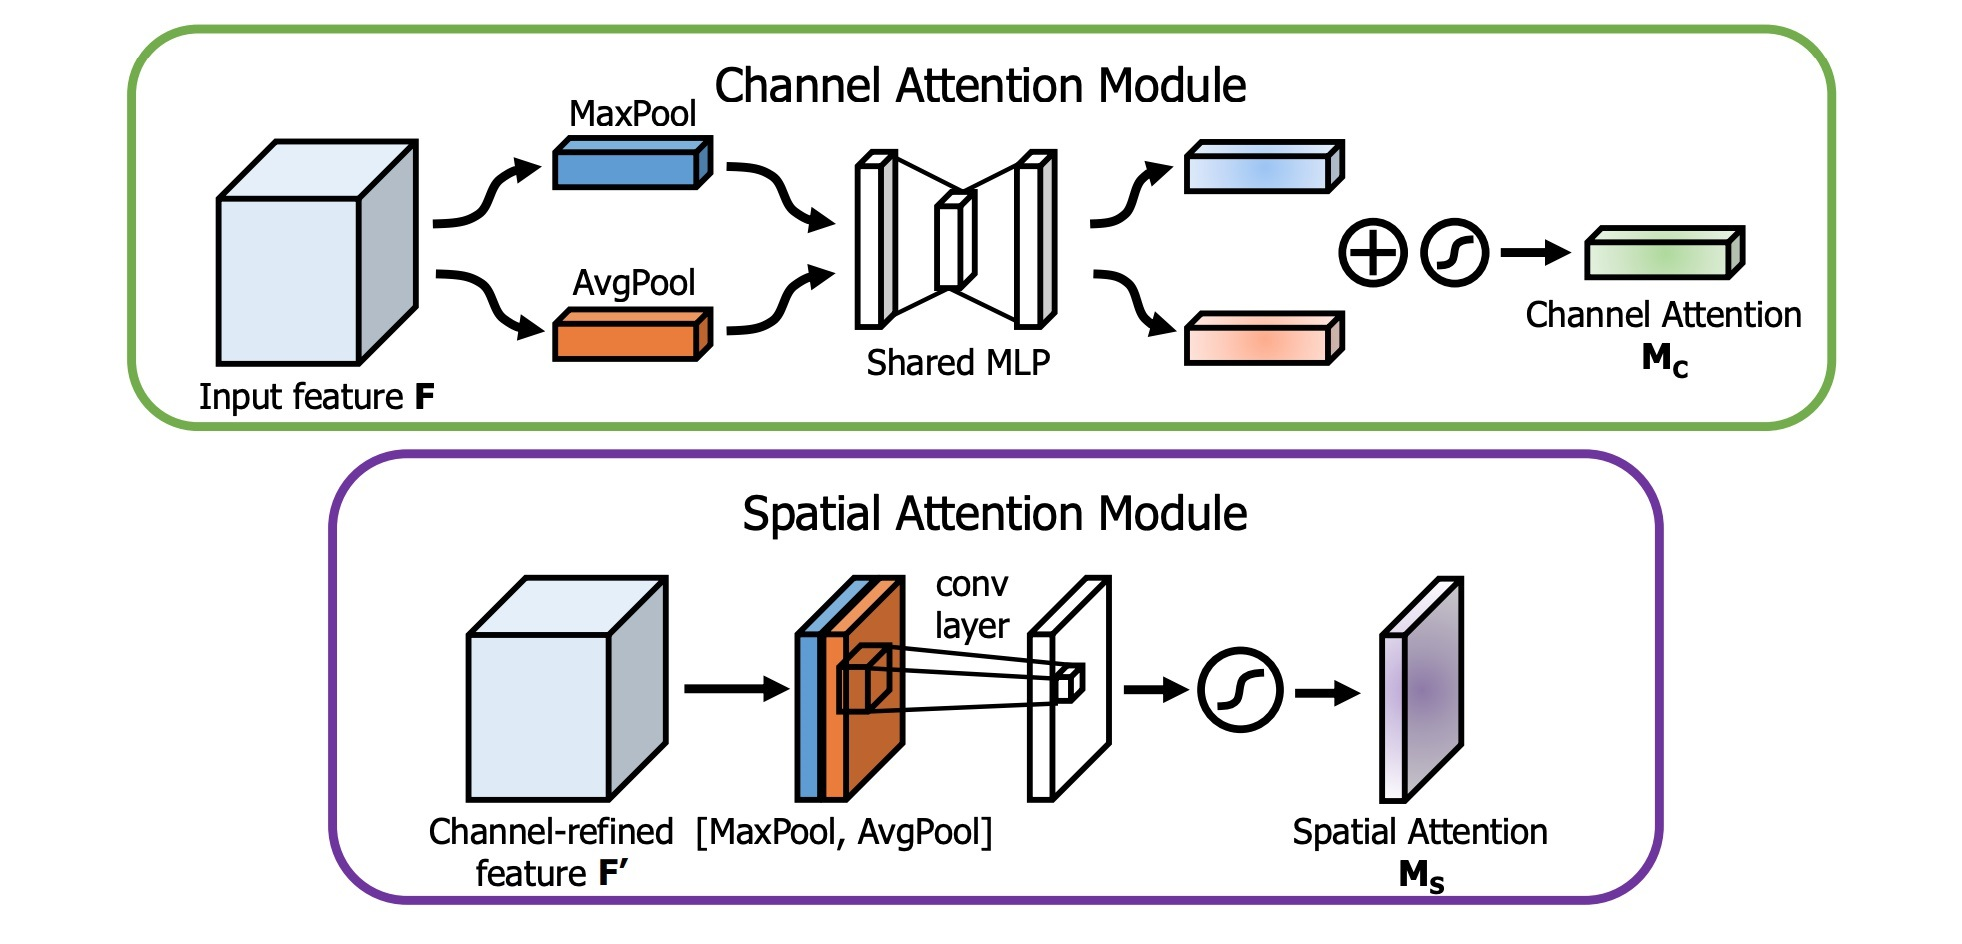
\includegraphics[scale=0.3]{cbam.jpg}
\caption{CBAM模块 示例}
\label{fig:cbam}
\end{figure}

\textbf{通道注意力模块} 通道注意力模块将输入$\mathbf{X}$分别进行平均池化和最大池化,输入共用的卷积层来实现通道注意力。如下是表达式:

$$\mathbf{M_c}(\mathbf{X})=\sigma(\mathrm{MLP}(\mathrm{AvgPool}(\mathbf{X}))+\mathrm{MLP}(\mathrm{MaxPool(\mathbf{X})}))$$

其中,$\mathrm{MLP}(\mathbf{X})=\mathbf{W_1}(\mathrm{ReLU}(\mathbf{W_0}(\mathrm{X})))$,$\mathbf{W_0},\mathbf{W_1}$都是权重。

\textbf{空间注意力模块} 空间注意力模块将通道注意力模块的输出特征图作为输入。分别做平均池化和最大池化后组合到一起(本次使用了加操作),再经过卷积降为1个通道。如下是表达式:

$$\mathbf{M_s}(\mathbf{X})=\sigma(\mathit{}{f}^{7\times 7}(\mathrm{AvgPool}(\mathbf{X})+\mathrm{MaxPool}(\mathbf{X})))$$

\subsection{损失函数}

再训练图像分类模型时,数据集各个分类的图像个数并不一定相等,如果数据集中某一类数量比较多,则训练完成后,网络倾向于将样本判断为该类。所以我们需要损失函数能够处理类别不平衡的情况。对于多分类交叉熵损失函数,我们可以使用何凯明等人提出的Focal Loss\cite{lin2017focal},该方法加入了描述样本分类的难易程度$r$和样本平衡因子$r$,对于样本$i$的损失函数为:

$$\mathrm{L}_i=\sum(-ay(1-y')^r\times\log(y')-(1-a)(1-y)y'^r\times\log(1-y'))$$

其中$y$是样本的标签,$y'$是logits。$r$标准值为0。$r$越大,模型对于预测值接近正确值的loss减小,而使预测值偏离正确值大的样本loss增大。$a$标准值为0.5。 $a$越大,模型对于预测准确率的敏感度越大;反之则对于错误率更敏感。

\subsection{数据增强方法}

数据增强指的是对数据做变换来增加训练数据的方法。深度学习需要大量数据进行训练,当数据略少时,可以使用翻转、平移、旋转、裁剪等方法,产生大量的新数据。使用此方法,可以使网络学到某一类的共性,而不是个别数据的特点而造成过拟合。

如图\ref{fig:data_augment},垃圾分类训练集原始图像通过随机平移、选择、缩放等技术,得到9张增强后的图片。

\begin{figure}[h!]
\centering
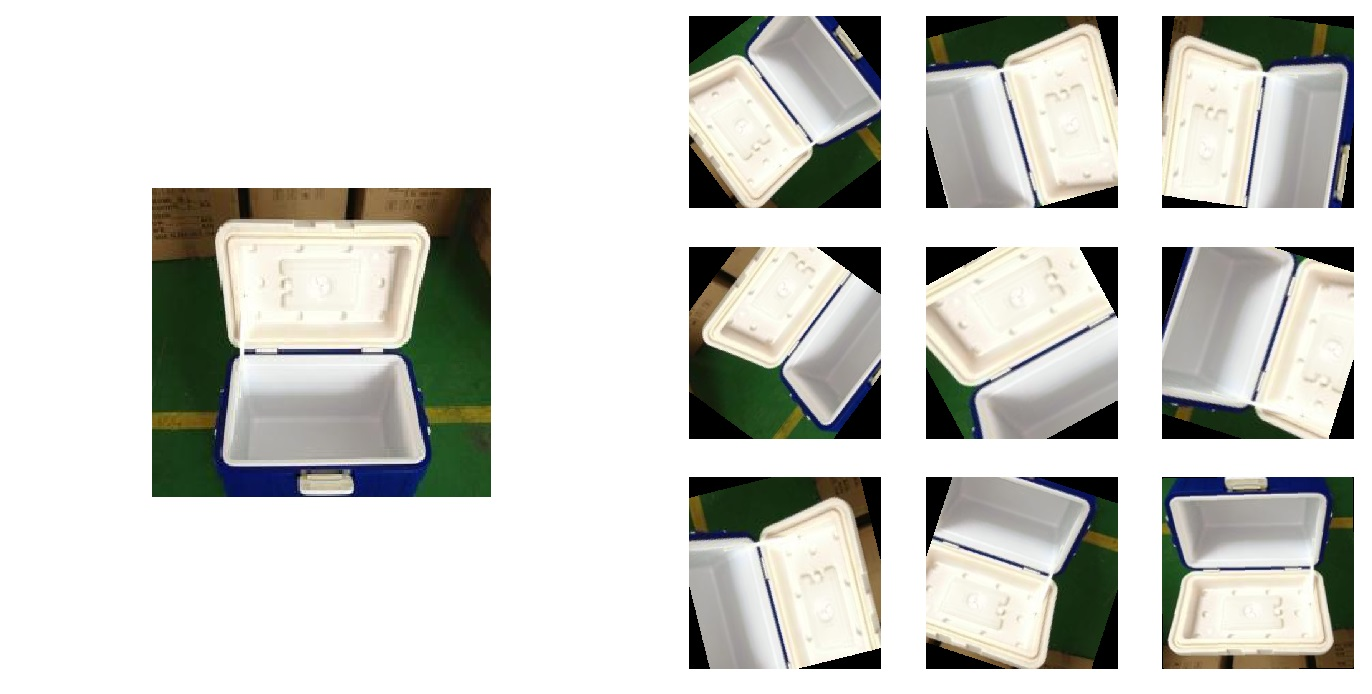
\includegraphics[scale=0.4]{data-augment.jpg}
\caption{数据增强示例}
\label{fig:data_augment}
\end{figure}

在实际使用过程中,由于拍摄设备设置等条件的限制,拍摄的垃圾图片可能不会处于中心的位置,视角也可能不在正对待分类物品的方向上。所以通过数据增强,可以得到更全面的物体特征,提高模型的鲁棒性。

\subsection{动态学习率}

学习率$\alpha$是神经网络训练中重要的超参数,在梯度下降法中,$\alpha$的取值更是至关重要的,过大过小会导致不收敛、收敛太慢的问题,而使用动态调整的学习率可以一定程度上增加学习效果。

\textbf{学习率预热}  在最初几轮迭代,模型得到的梯度往往很大,为避免训练不稳定,可以使最初几轮迭代采用较小的学习率:$$\alpha_t'=\frac{t}{T'}\alpha_0,\ \ 1\leq t\leq T'$$
其中$\alpha_0$是初始学习率,$T'$是预热的迭代次数。预热结束后,再开始使用一种学习率衰减:

\textbf{学习率衰减}  一般来说,训练刚开始时学习率要大写来寻找最值点、保证收敛速度,而到收敛到最优值附近时学习率则要小一些避免损失震荡。可以使用学习率衰减的方法实现逐渐减小学习率,学习率衰减有以下几种:

\begin{enumerate}
    \item 分段常数衰减(Step Decay):经过第$i$次迭代,学习率乘上系数$\beta_i$,其中$\beta_i<1$为超参数。
    \item 指数衰减(Exponential Decay):$\alpha_i=\alpha_0\beta^i$
    \item 余弦衰减(Cosine Decay): $\alpha_i=\frac{1}{2}\alpha_0(1+\cos(\frac{i\pi}{T}))$,其中$T$是总的迭代次数。
\end{enumerate}

% 为什么使用动态学习率,使用什么样的动态学习率。如

\subsection{标签平滑技术}

\section{实验}
\subsection{实验设置}

本文采用华为垃圾分类挑战杯数据集,该数据集包括厨余垃圾、可回收物、其他垃圾、有害垃圾4大类,每个大类由若干小类,共计40个小类,共计14800张图片。采用4:1的训练-测试划分。可选择是否进行数据增强,若使用,每张图片随机经过随机翻转、随机裁剪等操作生成5张图片。

本文实验使用Pytorch版本为1.6.0,总共构建了ResNet三个不同深度的模型:

ResNet18,ResNet50,ResNet101,和它们相对应的使用CBAM的模型进行了实验。在模型中使用了Pytorch预训练的参数。\footnote{https://github.com/s7a9/GarbageClassification.git}

\subsection{实验结果}
不同模型、有无图像增强方法、不同学习率策略、标签平滑技术,各种情况下与baseline的效果对比。

不同垃圾类别上的精度。

一些badcase的分析。
\section{结束语}
本文尝试了……

实验发现……效果比较好。

未来可以尝试更多方向……

\bibliographystyle{plain}
\bibliography{references}

\end{CJK*}

\end{document}
